\documentclass{article}
\usepackage[spanish]{babel}
	\deactivatetilden
\spanishdecimal{.}
\addto\captionsspanish{\def\tablename{Tabla}}
\addto\captionsspanish{\def\listtablename{\'Indice de tablas}}
\usepackage[numbers,sort&compress]{natbib}
\usepackage[T1]{fontenc}
\usepackage[utf8]{inputenc}
\usepackage{graphicx}
\usepackage{url}
\usepackage{graphicx}
\graphicspath{{Figuras/}}
\usepackage[numbers,sort&compress]{natbib}
\usepackage[clearempty,pagestyles]{titlesec}
\usepackage{anysize}

\def\baselinestretch{1.5}
\papersize{27.9cm}{21.5cm} 
\marginsize{2cm}{2cm}{1cm}{1cm}

\title {Teoría de colas}
\author{Julio Garc\'ia}


\pagestyle{empty}

\begin{document}

\maketitle

\section{Introducción}

En el presente trabajo se busca como objetivo principal el estudio de la Teoría de Colas, en esta área se conocen un sinfín de aplicaciones en la vida real. Algunos de los procesos de líneas de espera más estudiados son:  filas de bancos, líneas de producción, servicios a clientes en telefonía y procesamientos de trabajos en servidores. Es evidente que el estudio de esta área tiene beneficios importantes, uno de ellos es el ahorro y estimación de tiempos. En la tarea \cite{p3}, se busca estudiar un proceso de línea de espera de procesamiento de trabajos (job) que son asignados y a su vez secuenciados en cada uno de los núcleos de una computadora. En particular, el trabajo a procesar es decidir si un número entero es un número primo. Se conoce como número primo, aquel número entero que sólo tiene como divisores exactos al uno y al mismo número. A continuación, se describe el problema a estudiar, se detalla la simulación para dicho problema y se presentan los resultados obtenidos.

\section{Desarrollo}
En este trabajo se busca analizar  el siguiente problema: Examina cómo las diferencias en los tiempos de ejecución de los diferentes ordenamientos cambian cuando se varía el número de núcleos asignados al cluster, utilizando como datos de entrada un vector que contiene primos grandes, descargados de https://primes.utm.edu/lists/small/millions/ y no-primos con por lo menos ocho dígitos. Investiga también el efecto de la proporción de primos y no-primos en el vector igual como, opcionalmente, la magnitud de los números incluidos en el vector con pruebas estadísticas adecuadas.\\
En base a lo propuesto en la tarea 3 por la Dra. Shaeffer \cite{p3}, es importante señalar que el procesamiento de los distintos trabajos (chambas) no están relacionados entre sí, esto permite la división (procesamiento) de cada uno de ellos en distintos núcleos. El código de este trabajo se realizó tomando como base el código propuesto en clase y se modificó de acuerdo con los objetivos señalados en la tarea.   

\section{Experimentación y resultados}

En esta sección se describe el ambiente computacional y los resultados obtenidos con la simulación. El código de dicha simulación fue realizado en el lenguaje computacional Python, en una computadora personal con procesador Intel Core i7, con memoria RAM de 16GB y hasta 8 núcleos de procesamiento. Dicho código fue incorporado en el repositorio \cite{p_3}. Para este estudio, se siguieron las recomendaciones propuestas por la Dra. Shaeffer \cite{pa}, por lo cual se decidió correr únicamente de uno a siete núcleos la experimentación. 

Los datos del experimento se tomaron del archivo Primes2.txt, el cual se descargo del link señalado en la tarea 3. De acuerdo con las recomendaciones propuestas en la clase, se decidió trabajar con trabajos difíciles y trabajos fáciles. Para el conjunto de trabajos difíciles, se obtuvieron los primeros 1710 números primos del archivo Primes2.txt, y para el conjunto de trabajos fáciles, se realizó la secuencia de los números enteros consecutivos iniciando con el primer digito del archivo Primes2.txt. En los trabajos fáciles, se tienen considerados números primos y números no primos, por lo cual se tienen trabajos que no consumen mucho tiempo. Por último, se siguió los ordenes propuestos en la tarea para el conjunto de datos, los cuales se basen en un orden ascendente, descendente y aleatorio del conjunto de datos a analizar.

La métrica por analizar es el tiempo promedio de realización de todos los trabajos resueltos en cada uno de los conjuntos de núcleos definidos, en una cantidad finita de replicas. La tabla 1 relaciona la cantidad de núcleos usados con el orden en que fueron ejecutados los trabajos, es decir, orden ascendente (menor a mayor), orden descendente (mayor a menor) y orden aleatorios. Además, se muestran los resultados de forma gráfica, indicando la tendencia que existe en los tiempos: 

\begin{center}
	\begin{tabular}{|c|c|c|c|}
		\hline
		Núcleos & Ascendente & Descendente & Aleatorio \\
		\hline
		1 & 0.16312 & 0.07348 & 0.06899 \\
		\hline
		2 & 0.16196 & 0.05678 & 0.05333 \\
		\hline
		3 & 0.18988 & 0.05334 & 0.04996 \\
		\hline
		4 & 0.20619 & 0.04968& 0.04673 \\
		\hline
		5 & 0.21399 & 0.04598 & 0.04353 \\
		\hline
		6 & 0.22059 & 0.04306 & 0.04086 \\
		\hline
		7 & 0.22136 & 0.04052 & 0.03854 \\
		\hline
	\end{tabular}
\end{center}
\begin{center}
	Tabla 1: Resultados trabajos faciles.
\end{center}

\begin{center}
\begin{tabular}{|c|c|c|c|}
	\hline
	Núcleos & Ascendente & Descendente & Aleatorio \\
	\hline
	1 & 0.80489 & 0.67855 & 0.66031 \\
	\hline
	2 & 0.65241 & 0.53013 & 0.51851 \\
	\hline
	3 & 0.56525 & 0.45374 & 0.44555 \\
	\hline
	4 & 0.51642 & 0.40052 & 0.39724 \\
	\hline
	5 & 0.485243 & 0.363248 & 0.36025 \\
	\hline
	6 & 0.46361 & 0.33489 & 0.33273 \\
	\hline
	7 & 0.44798 & 0.31312 & 0.31039 \\
	\hline
\end{tabular}
\end{center}
\begin{center}
	Tabla 2: Resultados trabajos diciles.
\end{center}

\begin{figure}
	\centering
	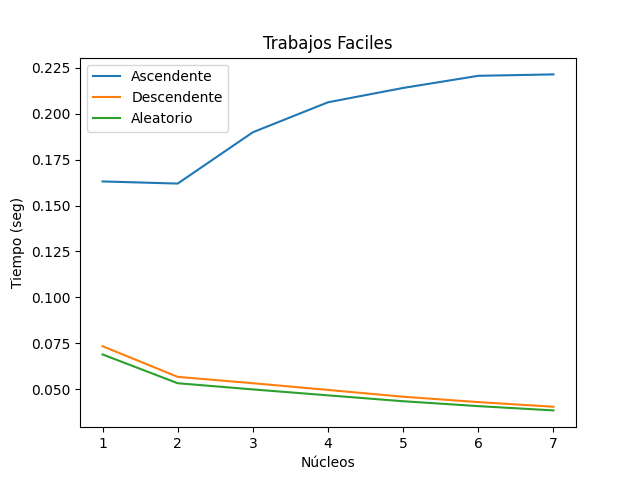
\includegraphics[width=0.7\linewidth]{Figure_1}
	\caption{Resultados trabajos faciles.}
	\label{fig:figure1}
\end{figure}


\begin{figure}
	\centering
	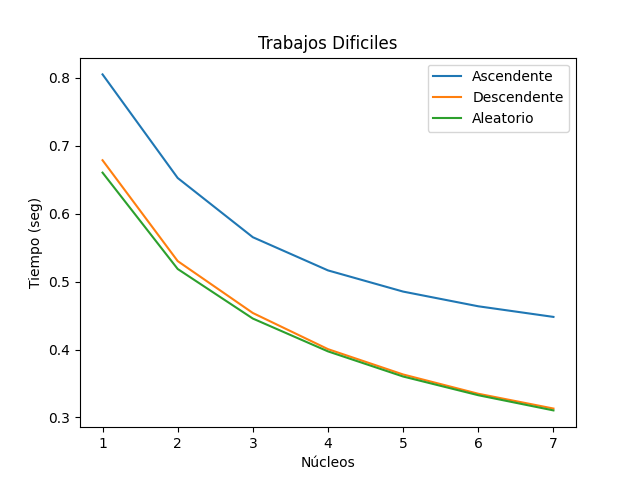
\includegraphics[width=0.7\linewidth]{Figure_2}
	\caption{Resultados trabajos dificiles.}
	\label{fig:figure2}
\end{figure}

\section{Conclusión}
Tomando como referencia el orden descendente de acuerdo con las tablas 1 y 2, presentadas en la sección anterior, se puede observar que existe una diferencia de tiempo significativa entre los trabajos difíciles y los trabajos fáciles. Esta diferencia es hasta 9 veces mayor el tiempo de las tareas difíciles comparado con las tareas fáciles. Además, se puede observar que la cantidad de tiempo va disminuyendo entre más se aumenta la cantidad de núcleos, es decir, es inversamente proporcional la cantidad de tiempo con respecto a la cantidad de nucleos. Estas conclusiones son iguales para el orden aleatorio. 
Por otra parte, el orden ascendente fue el que se tardo más tiempo en procesar todas las tareas, además de presentar un comportamiento atípico en el crecimiento de tiempos al ir aumentando la cantidad de núcleos. Por lo anterior, si se desea realizar la simulación en un ambiente computacional similar y tardar el menor de los tiempos, se recomienda usar el orden descendente (inverso) y usar la mayor cantidad de núcleos.

\bibliography{Biblio}
\bibliographystyle{plainnat}

\end{document}